\section{Loading a Kernel}
As seen in the Programming Model chapter, host programs can upload kernels to the GPU.
They should preferably do so at the beginning of the program, to avoid delays during execution.

The CPU's Demolicious library has a built-in function for this called \verb/load_kernel/, seen in listing \ref{lst:load-kernel}.
It takes an array of assembled instructions as parameter,
allocates memory on the GPU and uploads the kernel,
before it returns a reference to GPU memory pointing to the start of the kernel.
This reference is used when starting kernels.

\begin{c-code}[caption=A load\_kernel function call with the fillscreen kernel, label=lst:load-kernel]
kernel_t fill_screen = load_kernel(fill_screen_kernel);
\end{c-code}

\begin{figure}[H]
    \centering
    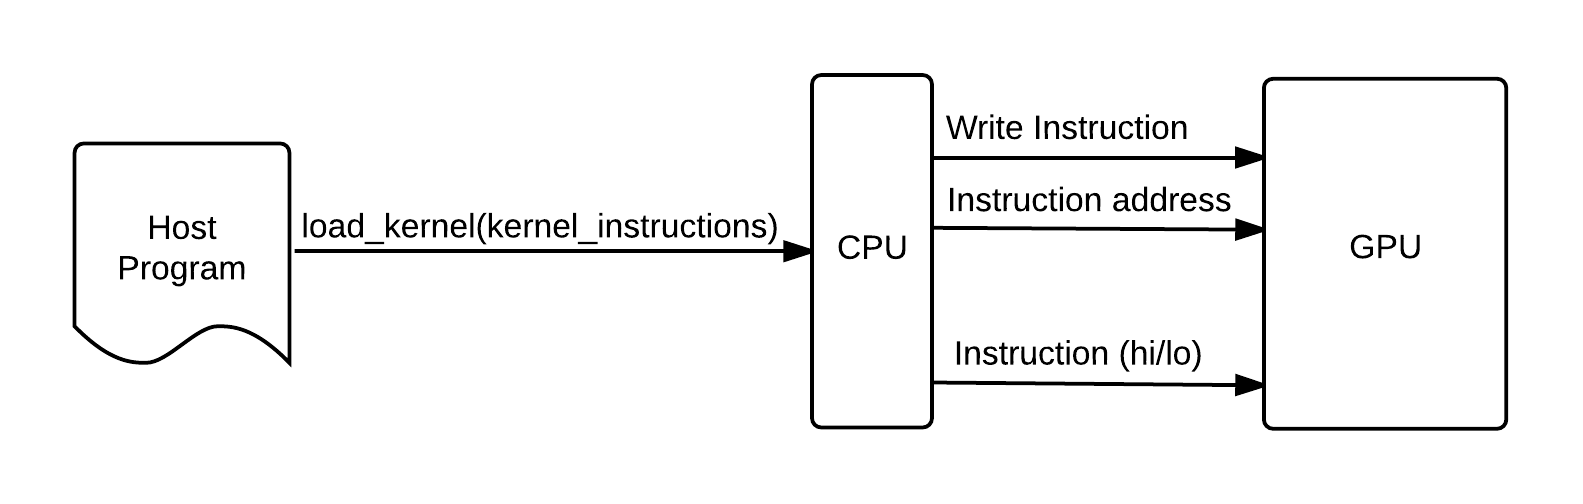
\includegraphics[width=\textwidth]{../cpu/diagrams/loading_a_kernel.png}
    \caption{}
    \label{fig:loading_a_kernel}
\end{figure}

Seeing as instructions are 32-bit large, and the data bus is only 16 bits,
every instruction load must be divided in two writes.
